\section{Use Case 2: Roadwarrior VPN}
In diesem Use Case soll erarbeitet werden, inwiefern sich Mitarbeiter via \gls{VPN} - im Folgenden \gls{Roadwarrior} genannt - mit den zuvor ausgerollten Cloud-Infrastrukturen verbinden können. Ralf Spenneberg definiert diesen Begriff wie folgt:\\
\glqq Der Begriff \gls{Roadwarrior} bezeichnet Personen, die mit unbestimmter IP-Adresse auf ein \gls{VPN-Gateway} zugreifen wollen. Typischerweise handelt es sich hierbei zum Beispiel um Außendienstmitarbeiter, die von unterwegs Zugriff auf die Datenbanken ihres Mutterunternehmens benötigen. Aber auch alle anderen Konstellation, bei denen Rechner mit dynamischen IP-Adressen eine \gls{VPN}-Verbindung mit einem \gls{VPN-Gateway} aufbauen möchten, sind denkbar. Hierbei ist die Anzahl der \gls{Roadwarrior} nicht beschränkt. Theoretisch und auch praktisch sind mehrere Hundert gleichzeitiger Tunnel möglich.\grqq{} \cite[S. 199]{Spenneberg2010}\\
Gerade die Corona-Krise hat das Ausweichen auf das Home-Office für einige Branchen unverzichtbar gemacht. Einige prophezeien bereits eine neue Arbeitswelt \textit{New Work}, die \glqq flexible Arbeitsgestaltung, zum Beispiel durch Vertrauensarbeitszeit und -orte sowie Verzicht auf standardisierte Kernarbeitszeiten\grqq{} mit sich bringt \cite{Umbs2020}.
Klassischerweise verbindet sich der \gls{Roadwarrior} mit dem Hauptstandort, um von dort aus weitere interne Ressourcen zu erreichen - in diesem Falle die Private Cloud. Dieses klassische Design bringt insbesondere unter der Annahme, dass sich Dienste in die Cloud verlagern lassen, diverse Probleme mit sich:
\begin{itemize}
\item Der Hauptstandort muss Bandbreite für alle $n$ \gls{Roadwarrior} zur Verfügung stellen. V.a. zu Beginn der Corona-Krise durften viele Unternehmen und öffentliche Einrichtungen erfahren, dass sie hier zu schwach aufgestellt sind \cite{tufreiberg2021}.
\item Der Hauptstandort ist u.U. weit entfernt. Der Mitarbeiter nimmt auf Grund von hohen Latenzen und eventuellen Paketverlusten eine schlechte Applikations-Performance wahr. Dazu wird oftmals über Smartphone-Hotspot, Hotel-WLAN, o.ä. gearbeitet, welche häufig eine unterdurchschnittliche Internetanbindung anbieten.
\item Latenzen erhöhen sich zusätzlich, falls bestimmte Applikations-Server gar nicht am Hauptstandort vorhanden sind, z.B. weil sie in die Public Cloud verlagert wurden.
\end{itemize}
Optimalerweise wird das Design also diese genannten Punkte in Angriff nehmen:
\begin{itemize}
\item Ein Lastenausgleich der Bandbreiten wird ermöglicht, indem $n$ \gls{Roadwarrior} über $m$ Clouds verteilt werden.
\item Der \gls{Roadwarrior} verbindet sich im günstigsten Fall mit dem Standort, der die geringste Entfernung zu ihm aufweist.
\item Häufig genutzte Applikationen sind am jeweiligen Cloud-Standort, mit dem sich der \gls{Roadwarrior} verbunden hat, verfügbar, um eine gute Usability für den Anwender zu gewährleisten.
\item Weiterhin sollen genannte Maßnahmen für den Anwender möglichst transparent und ohne manuelle Interaktion erfolgen. Er soll keine Wahl haben, mit welchem Cloud-Standort er sich zu verbinden hat: Die Annahme ist, dass dieser über geeignete Automatisierungsmechanismen mit dem \textit{besten} Standort verbunden wird.
\end{itemize}
Das Szenario baut auf Use Case 1 auf. So wird weiterhin von dem Backbone-Grundaufbau ausgegangen. Es soll gezeigt werden, wie ein \gls{Roadwarrior}-Setup aufgebaut werden kann, bei dem sich der jeweilige Mitarbeiter mit dem nächstgelegen \gls{VPN-Konzentrator} verbindet, um die beste Performance erreichen zu können.\\
Weiterhin soll an jedem Cloud-Standort ein Server stehen, welcher einen \textbf{internen} Netzwerk-Dienst anbietet. Das Ziel ist es, dass ausschließlich der interne Server genutzt wird, der an dem Standort zur Verfügung steht. Ansonsten würde sich der Latenzgewinn des nahen \gls{VPN-Konzentrator}s durch die \textit{interne} Latenz des Backbones wieder aufheben.\\
Die Infrastruktur aus Use Case 1 wird als vorhanden und funktionierend angenommen und in Abbildung \ref{grafik:Use-Case-2_Vereinfacht} nicht mehr dargestellt.
\begin{figure}[h]
  \centering
  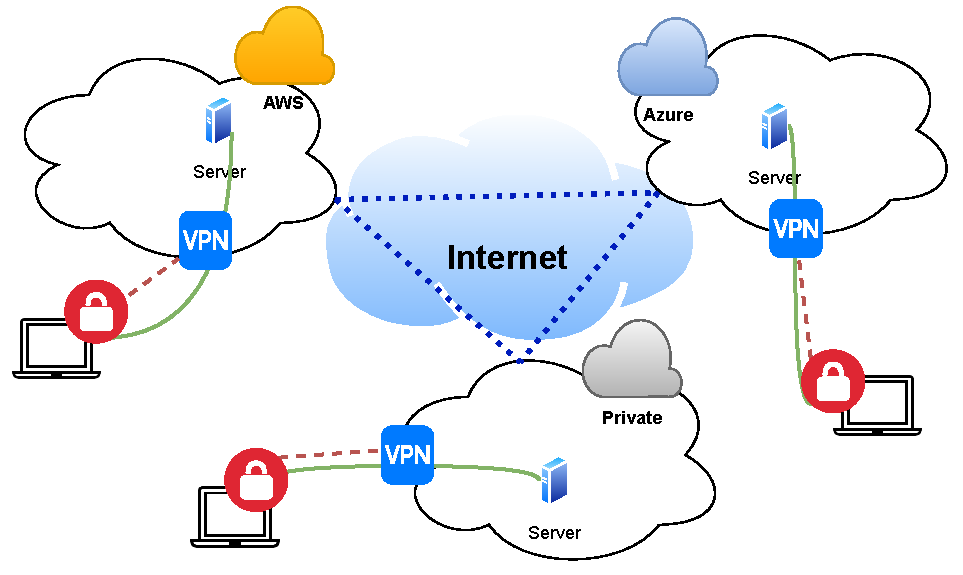
\includegraphics[scale=0.75]{Figures/Use-Case_2_Vereinfacht_1.pdf}
  \caption{Use Case 2: Roadwarrior}
  \label{grafik:Use-Case-2_Vereinfacht}
\end{figure}\FloatBarrier

\subsection{Vorauswahl geeigneter technischer Komponenten}\label{uc1-vorauswahl}
Zur Terminierung der \gls{Roadwarrior}-\gls{Client}s muss pro Cloud-Standort ein \gls{VPN-Konzentrator} zur Verfügung stehen. Mit \textit{\gls{Client} \gls{VPN} Endpoint} (AWS) bzw. \textit{Point-to-site} Azure werden von den Cloud-Providern bereits Lösungen angeboten, um \gls{Roadwarrior}-\gls{Client}s zu terminieren. Nach längerer Evaluation dieser Building Blocks erwiesen sich diese Lösungen für das Ziel der Arbeit als nicht tauglich:
\begin{itemize}
\item Bei AWS werden \gls{Client-to-Site}-Verbindungen eingehend ge\gls{NAT}ted (\textit{NAT Masquerading}). Damit sind alle \gls{Client}s intern mit der gleichen Absender-IP zu sehen. Dies verletzt den Anspruch der Arbeit, eine Ende-zu-Ende-Konnektivität zu ermöglichen.
\item Obwohl Azure als auch AWS OpenVPN für \gls{Roadwarrior}-\gls{VPN}s benutzen, sind die \gls{Client-to-Site}-Konfigurationen nicht \glqq deckungsgleich\grqq{} zu bekommen. Um sich mit dem nächstgelegenen \gls{VPN-Konzentrator} zu verbinden, wäre eine manuelle Interaktion des Benutzers notwendig, was mit den Evaluationskriterien nicht vereinbar ist (s. Kap. \ref{eval-roadwarrior}). Weiterhin kann der Benutzer nicht immer wissen, wo der nächstgelegene Standort ist. Man kann nicht von jedem Mitarbeiter tiefe Kenntnisse der Netzwerktopologie abverlangen.
\end{itemize}
AWS benutzt bspw. eine \textit{remote-random-hostname}-Direktive (s. Listing \ref{ovpn-client-config-remote}), welche dafür sorgt, dass bei Verbindungsversuch eine Zufallszeichenkette an den Domainnamen angehangen wird, um \gls{DNS} Caching zu verhindern.
%TC:ignore
\begin{listing}[h]
\begin{minted}[breaklines,frame=single]{bash}
$ grep remote *-client-vpn.ovpn
aws-client-vpn.ovpn:remote cvpn-endpoint-08345.prod.clientvpn.eu-central-1.amazonaws.com 443
aws-client-vpn.ovpn:remote-random-hostname
aws-client-vpn.ovpn:remote-cert-tls server
azure-client-vpn.ovpn:remote azuregateway-61820068.vpn.azure.com 443
azure-client-vpn.ovpn:remote-cert-tls server

\end{minted}
\caption{Auszüge aus den OpenVPN-Client-Konfigurationen für AWS und Azure}
\label{ovpn-client-config-remote}
\end{listing}\FloatBarrier
%TC:endignore
Weiterhin sind die unterschiedlichen Authentifizierungsmechanismen nur schwierig miteinander zu kombinieren. Auch hier wäre eine Benutzerinteraktion notwendig.\\
Daher wurde für weitere Überlegungen von den offiziellen Building-Blocks abgesehen und entschieden, pro Standort einen eigenen OpenVPN-Server hochzufahren: OpenVPN ist freie Software und man muss sich daher nicht mit Lizenzierungen beschäftigen analog zu VyOS.\\
Aus den Erfahrungen aus Use Case 1 wurde dafür ebenso die Router-Distribution VyOS gewählt. Diese kann nicht nur für \gls{Site-to-Site}-Tunnel genutzt werden, sondern kann auch für \gls{Client-to-Site}-Tunnel terminieren, um den Zugang für \gls{Roadwarrior} zu ermöglichen.\\
Denkbar wäre ebenso eine simple Linux-Distribution mit dem Paket OpenVPN: VyOS bietet den Vorteil, dass sich die notwendigen Konfigurationen ebenso über CLI erledigen lassen und somit per Terraform-Template \textit{automatisiert} ausgebracht werden können\cite{vyosopenvpn2021}. VyOS ist im AWS als auch im Azure Marketplace zu beziehen.\\
Ein Problem ergibt sich aus der Authentifizierung und Autorisierung der \gls{Roadwarrior}-\gls{Client}s. Wenn Protokolle wie RADIUS\cite{rfc2865} als Authentifizierungsmechanismus mit Benutzerkennung und Passwort, muss man entweder
\begin{enumerate}[label=(\alph*)]
\item \label{radius-decentralized} einen zentralen RADIUS-Server pro Standort verwalten oder
\item \label{radius-centralized} einen zentralen RADIUS-Server für alle Standorte zur Verfügung stellen.
\end{enumerate}
\ref{radius-decentralized} bringt ein Skalierungsproblem mit sich: So müssen bspw. Benutzerkennungen und Passwörter lokal auf allen Systemen gepflegt werden, was die Komplexität des Use Cases deutlich erhöhen würde und auch in Realität schwierig zu warten wäre. Mit \ref{radius-centralized} hätte man einen Single-Point-of-Failure und scheidet somit auch aus. Hätte der \textit{zentrale} Authentifizierungsserver ein technisches Problem, wären alle \gls{VPN-Konzentrator}en betroffen und \gls{Roadwarrior} könnten sich nicht mehr verbinden.\\
Lightweight Directory Access Protocol (LDAP)\cite{rfc4511} als verteilte Datenbank wäre eine Lösung für genannte Probleme: man müsste pro Standort einen LDAP-Server bereitstellen und durchgehend mit allen weiteren LDAP-Servern synchronisieren. Als Authentifizierungsmechanismus könnte man dann bspw. RADIUS\cite{rfc2865} oder gleich LDAP benutzen. \textit{Windows Domänen Controller} implementieren den LDAP-Verzeichnisdienst in Form von \textit{Active Directory} und wären ein Beispiel für solch ein verteiltes Szenario.\cite[S.603-604]{Tanenbaum2003}\\
In dieser Arbeit wird von der Implementation abgesehen, da die Komplexität deutlich erhöht und diese für den Proof of Concept an sich keine gewinnbringenden Erkenntnisse liefern würde.\\
Der Lösungsansatz ist an dieser Stelle, auf eine Zertifikat-basierte Authentifizierung zu setzen. Eine Public-Key-Infrastruktur (PKI) benötigt zur Authentifizierung keine Verbindungen zu anderen (Authentifizierungs-)Services. Es reicht, auf dem \gls{VPN-Konzentrator} vertrauenswürdige Root-Zertifikate zu hinterlegen. Diese \textit{vertrauenswürdigen Stellen} signieren mit dem privaten Schlüssel dann die Zertifikate der \gls{Roadwarrior}-\gls{Client}s, wodurch das Vertrauensverhältnis zwischen VPN-Server und -\gls{Client} hergestellt ist.\\ 
Auf Prüfung der Gültigkeit von Zertifikaten mittels Certificate Revocation Lists (CRLs) bzw. Online Certificate Status Protocol (OCSP) wird in dieser Arbeit verzichtet. Sie ist aber prinzipiell möglich mit der serverseitigen OpenVPN-Direktive \textit{crl-verify} (CRL-Prüfung) bzw. \textit{tls-verify} (OCSP-Prüfung).\cite[S.116, S.325-327]{Keijser2011}\\
%tf remote
Als \gls{PKI} wird eine pfSense-Instanz genutzt. Dieses Firewall-Betriebssystem bietet eine simple \gls{PKI}, welche via Web-GUI administrierbar ist und so das Ausstellen und die Verwaltung der \gls{Client}- und Server-Zertifikate erleichtert.\cite[S.376-383]{Netgate2020}\\
Der technische Fokus wird in diesem Use Case auf \gls{DNS} liegen. Es soll in dem Szenario zwei essenzielle Aufgaben lösen, die durch die Evaluationskriterien (s. Kap. \ref{eval-roadwarrior}) vorgegeben werden:\label{evalkriterien-uc2}
\begin{enumerate}
\item Mit Hilfe von \gls{GeoIP}-Daten soll ermöglicht werden, immer den nächstgelegenen \gls{VPN-Konzentrator} zu finden.\label{geoip-nearest-vpn}
\begin{enumerate}[label=(\alph*)]
    \item Wenn ein Server in der Nähe ist, soll dieser kontaktiert werden.\label{server-nearest}
    \item Wenn kein Server in der Nähe ist, soll ein beliebiger Server kontaktiert werden (\textit{random})\cite{bindrrset2020}.\label{no-server}
    \item Wenn das Terraform \gls{Deployment} noch nicht stattgefunden hat, also keine Public Cloud-Standorte zur Verfügung stehen, soll sich der \gls{Client} immer mit dem \gls{VPN-Konzentrator} der Private Cloud verbinden.\label{server-not-deployed}
\end{enumerate}
\item Sobald der \gls{Roadwarrior} mit einem \gls{VPN-Konzentrator} verbunden ist, soll immer der (beispielhafte) Server, der am jeweiligen Standort bereitgestellt wurde, kontaktiert werden.
\end{enumerate}

Um die unterschiedlichen Fälle aus \ref{geoip-nearest-vpn} zu verdeutlichen, wurden zwei Entscheidungsbäume entwickelt. Der Server-seitige Fall der \gls{DNS}-Auflösung wird in Abb. \ref{grafik:Use-Case_2_Entscheidungsbaum_GeoIP} aufgezeigt.
\begin{figure}[h]
  \centering
  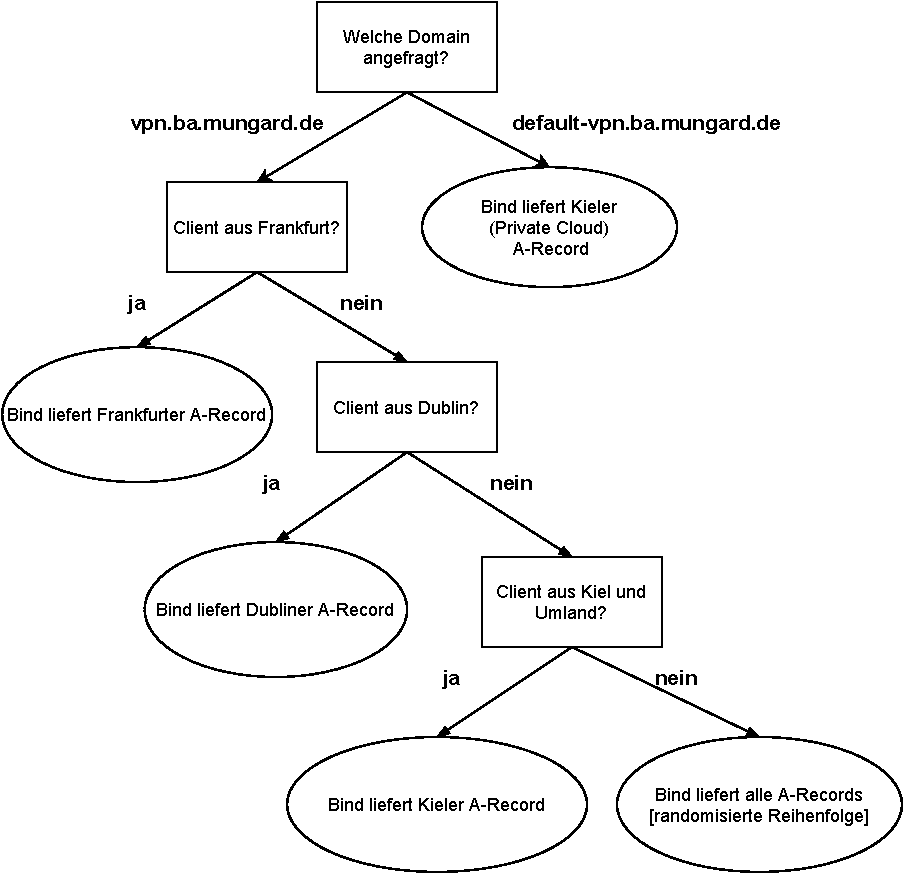
\includegraphics{Figures/entscheidungsbaum_bind_geoip.pdf}
  \caption{Entscheidungsbaum: Antwort des Nameservers für Zone ba.mungard.de}
  \label{grafik:Use-Case_2_Entscheidungsbaum_GeoIP}
\end{figure}\FloatBarrier

Fall \ref{server-not-deployed} ist \gls{Client}-seitig gesteuert und kommt dann zum Tragen, wenn der \gls{FQDN} vpn.ba.mungard.de nicht auflösbar sein sollte (s. Abb. \ref{grafik:Use-Case_2_Entscheidungsbaum_OpenVPN}).

\begin{figure}[h]
  \centering
  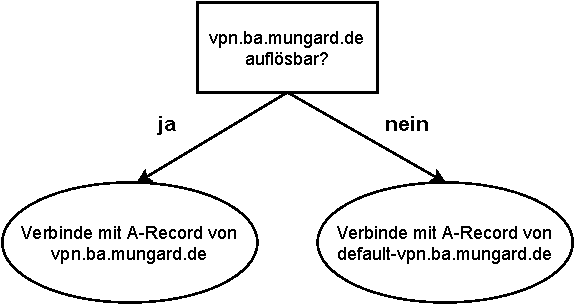
\includegraphics{Figures/entscheidungsbaum_openvpn_config.pdf}
  \caption{Entscheidungsbaum: DNS-Auflösung für Roadwarrior-VPN}
  \label{grafik:Use-Case_2_Entscheidungsbaum_OpenVPN}
\end{figure}\FloatBarrier

Mit Hilfe des Bind Nameservers ab Version 9.10 ist es möglich, die \gls{GeoIP}-Datenbank des Anbieters MaxMind auszuwerten, um \gls{DNS}-Anfragen in Abhängigkeit der Absender-IP zu beantworten\cite{bindgeoip2020}. Bei dieser IP handelt es sich typischerweise um die Resolver-IP des \textit{lokalen} Internet-Dienstleisters. Die Annahme für diesen Use Case ist daher, dass der \gls{DNS}-Resolver in der gleichen Region wie der \gls{Roadwarrior} angesiedelt ist\label{dns-resolver-region}.\\
Um mit \gls{GeoIP}-Daten der Firma MaxMind arbeiten zu können, muss Bind (Linux-Binary: \texttt{named}) mit einem speziellen Flag (\texttt{-{}-with-maxminddb}) kompiliert werden. Im Ubuntu 20.04 Standardpaket von Bind 9 ist dieses Feature bereits vorhanden (s. Listing \ref{bind-mmdb-compiler-flag}).

%TC:ignore
\begin{listing}[h]
\begin{minted}[breaklines,frame=single]{bash}

$ named -V | grep -o -- '--with-maxminddb'
--with-maxminddb

\end{minted}
\caption{\texttt{named} Compiler-Flags (gefiltert)}
\label{bind-mmdb-compiler-flag}
\end{listing}
%TC:endignore
Der Nameserver muss sowohl extern, also aus dem Internet, als auch intern für verbundene VPN-\gls{Client}s, erreichbar sein. Der Nameserver wird ausschließlich in der Private Cloud gehostet. Es wird von einem \gls{Deployment} eines \textit{secondary} Nameservers \textit{pro} Standort \gls{Deployment}s abgesehen. Es sind keine Erkenntnisgewinne dadurch gegeben. Secondary Nameserver halten Kopien aller \gls{Zone}n des primary Nameservers vor, welcher für die Verwaltung von \gls{Zone}ndateien zuständig ist\cite[S.517]{Fall2011}.\\
In der Praxis sollte das \gls{Deployment} von \glqq Secondaries\grqq{} aus Redundanzgründen jedoch dringend in Betracht gezogen werden. Außerdem können \glqq verzögerte\grqq{} \gls{DNS}-Antworten auf Grund sehr großer Entfernungen negative Auswirkungen auf die Usability haben. Da alle Test-Standorte innerhalb von Europa liegen, ist dieser Effekt im Sinne des Proof of Concepts vernachlässigbar.\\
Es müssen \gls{Zone}n dynamisch editierbar sein, da durch das Terraform-\gls{Deployment} virtuelle Maschinen mit vorher unbekannten IP-Adressen erstellt werden. Diese IP-Adressen müssen den jeweiligen \gls{Zone}n des autoritativen Nameservers bekannt gemacht werden. Dies gilt für extern und intern auflösbare \gls{Zone}n. Für Terraform steht ein Provider \textit{dns} zur Verfügung, der diese dynamischen Updates erlaubt\cite{dnstf2021}.
Das in diesem Kapitel angedeutete Szenario soll wieder per Terraform bereitgestellt werden und setzt direkt auf Use Case 1 auf. Auf Grund der langen Dauer des \gls{Deployment}s in Use Case 1 (siehe Kap. \ref{azure-deployment-time}) wird erwogen, Use Case 2 nicht \glqq komplett\grqq{} auszurollen, sondern Use Case 1 zu belassen und die Infrastruktur-Komponenten aus Use Case 2 lediglich hinzuzufügen (vgl. Kap. \ref{accelerate-deployment-use-case-2}).\\
Die OpenVPN-Server sollen auflösbar sein unter der Domain vpn.ba.mungard.de.\\
Als stellvertretender \glqq Applikations-Server\grqq{} soll ein Apache2-Webserver pro Standort in einer Ubuntu-\gls{VM} installiert werden. Dieser soll über die Domain www.intern.ba.mungard.de erreichbar sein.
\subsection{Evaluationskriterien}\label{eval-roadwarrior}
\begin{enumerate}
\item \gls{Roadwarrior}-\gls{Client}s werden simuliert, indem an den entsprechenden Standort (Kiel, Dublin bzw. Frankfurt) eine weitere virtuelle Maschine installiert wird, die \gls{VPN}-Ver\-bin\-dungen zu den jeweiligen \gls{VPN-Konzentrator}en aufbaut.
\item Ein \gls{Roadwarrior}-\gls{Client} verbindet sich immer mit dem nächstgelegen Standort. Die \gls{DNS}-Antworten werden per \texttt{dig}- und \texttt{whois}-Kommando verifiziert.
\item Der \gls{Client} hat keine Wahl, mit welchem Standort dieser verbunden wird.
\item Ist ein Cloud-Standort nicht verfügbar (z.B. weil defekt oder nicht bereitgestellt), \textit{muss} der \gls{Client} auf den \textit{default} Standort (Kiel) zurückfallen.
\item Sobald ein \gls{Client} mit einem \gls{VPN} verbunden ist, muss er die entsprechende interne Server-Ressource ansprechen, die am jeweiligen Standort zur Verfügung steht.
\end{enumerate}

Weitere Evaluationskriterien sind in der Praxis denkbar, spielen im Kontext des \textit{Proof of Concepts} dieser Arbeit jedoch keine Rolle.
